\section{Integralrechnung \formelbuch{493}}
			
	\subsection{Integrationsregeln \formelbuch{496ff und letzte Seite}} %Seitenzahlen OK 10 Auflage
	
	%TODO: verständlicher umschreiben
	\renewcommand{\arraystretch}{2}
	
		\begin{tabular}{|l|l|}
			\hline
			Linearit\"at & $\int{f(\alpha x+\beta )dx=\frac{1}{\alpha}\cdot F(\alpha x+\beta)+C}$ \\ \hline
			Summenregel & $ \int{\left(f(x) + g(x) \right)} dx = \int f(x) dx + \int g(x) dx $ \\ \hline
			Faktorregel & $ \int n \cdot f(x) dx = n \cdot \int f(x) dx $ \\ \hline
			Potenzregel & $ \int x^n dx = \frac{1}{n+1} \cdot n^{n+1} + C \qquad (n \neq-1) $ \\ \hline
			Partielle Integration & $\int\limits_a^b{u'(x)\cdot v(x)dx}=\biggl[u(x)\cdot v(x) \biggr]_a^b-\int\limits_a^b{u(x)\cdot v'(x)dx}$ \\ \hline
			Rationalisierung / & $t=\tan\frac{x}{2} \iff
			\frac{dx}{dt}=\frac{2}{1+t^2} \iff dx=\frac{2dt}{1+t^2} \qquad \sin(x)=\frac{2t}{1+t^2} \qquad \cos(x)=\frac{1-t^2}{1+t^2}
			$ \\
			Weierstrass-Substitution & $ \tan(x)=\frac{2t}{1-t^2} \iff \cot(x)=\frac{1-t^2}{2t} \hspace{10em} \int{R(\sin(x)\cos(x))dx} $ \\ \hline
			Allgemeine Substitution &
			$\int\limits_{a}^{b}{f(x)dx}=\int\limits_{g^{-1}(a)}^{g^{-1}(b)}{f(g(t))\cdot
				g'(t)dt}\qquad t=g^{-1}(x)\qquad  $\\ 
			 & $ z=g(t) \iff \frac{dz}{dt} = g'(t) \iff dt = \frac{dz}{g'(t)} dt$\\
			\hline
			Logarithmische Integration & $\int{\frac{f'(x)}{f(x)}dx}=\ln|f(x)|+C 
			\qquad{(f(x)\neq 1)}$\\ \hline
			Differentiation & $\int \limits ^{b} _{a} {f'(t)dt}=f(b)-f(a) \qquad \qquad \qquad \qquad \frac{d}{dx} \int \limits ^{x} _{1} {f(t)dt} = f(x)$ \\ \hline
			Spezielle Form des Integranden & 
			$\int{f'(x)\cdot
				(f(x))^{\alpha} dx}= f(x)^{\alpha +1}\cdot \frac{1}{\alpha+1}+C
			\qquad{(\alpha \neq -1)}$\\ \hline
	%		Mittelwerte & linear: $\frac{1}{b-a} \int_{a}^{b} f(x) d x \quad$ quadratisch: $\sqrt{\frac{1}{b-a} \int_{a}^{b}\left|f(x)^{2}\right| d x}$ \\ \hline
		\end{tabular}
	
	\renewcommand{\arraystretch}{1}
			



	\subsection{Uneigentliches Integral \formelbuch{519ff}} %Seitenzahlen OK 10 Auflage
	%TODO: weisser Platz auffüllen/ kompakter schreiben
	%TODO: verständlicher umschreiben und von anderen Formelsammlungen ergänzen
	%TODO: Inhalt ergänzen mit Bilder und Text aus Mendez - Skript S.19-22:
	  Uneigentliches Integral heisst, dass entweder eine \textbf{unbeschränkte
	  Funktion} integriert wird, oder eine Funktion über einen
	  \textbf{unbeschränkten Integrationsberech} integriert wird.\\
	
		\begin{itemize}
			\setlength{\itemsep}{1pt}
			\setlength{\parskip}{0pt}
			\setlength{\parsep}{0pt}
			
		  	\item $f(x)$ auf abgeschlossenem Intervall definiert, aber \textbf{nicht}
		  	beschränkt.
			\item $f(x)$ auf abgeschlossenem Intervall definiert mit Ausnahme eines
			Punktes.
			\item $f(x)$ hat eine	 Unendlichkeitsstelle.
		\end{itemize}
	
	
	  \begin{multicols}{2}
	    F\"ur unbeschr\"ankte Funktionen:\\
	    $ I =\int\limits _{a}^{c}f(x)dx=\lim\limits_{t\to
	    b-}\int\limits_{a}^{t}f(x)dx+\lim\limits_{t\to b+}\int\limits_{t}^{c}f(x)dx
	    $ \\
	    F\"ur die unbeschr\"ankte Integration:\\
	    $ I =\int\limits _{a} ^{\infty} f(x)dx= \lim \limits_{t\to \infty}\int \limits
	    _{a} ^{t}f(x)dx; $ \\
	    $ I =\int\limits ^{a} _{-\infty} f(x)dx= \lim \limits_{t\to -\infty}\int
	    \limits _{t} ^{a}f(x)dx; $ \\
	    $I =\int\limits _{-\infty} ^{\infty} f(x)dx = \lim \limits_{t_1\to \infty} \lim
	    \limits
	    _{t_2 \to  \infty}\int \limits _{t_1} ^{a}f(x)dx +
	    \int\limits_{a}^{t_2}f(x)dx$\\
	    Beispiel: $\int\limits_{1}^{\infty}\frac{1}{x^2}dx=\lim\limits_{t\to
	    \infty}\int\limits_{1}^{t}\frac{1}{x^2}dx=\lim\limits_{t\to \infty}-\frac{1}{t}+\frac{1}{1}=1$
	    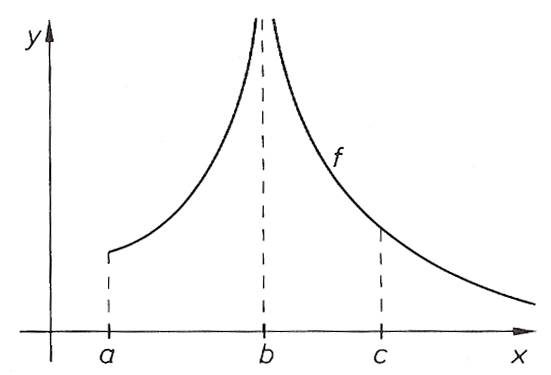
\includegraphics[width=4.5cm]{./bilder/unbeschraenkteFunktion.png}\\
	    unbeschr\"ankte Funktion
	  \end{multicols}
	  
	  
	    
	    
	\subsubsection{Prinzip der Restfl\"ache}
	  Wenn $\lim\limits_{t \rightarrow \infty} \int\limits^{\infty}_{t} f(x) dx = 0$, dann konvergiert
	  $\int\limits_a^{\infty} f(x) dx$ und umgekehrt.
	
	\subsubsection{Majorantenprinzip (konvergent)}
	  Um nachzuweisen, ob eine Funktion $|f(x)| \geq 0$ konvergiert, wird eine zweite
	  Funktion $g(x) \geq |f(x)|$ (Majorante) gesucht. Konvergiert $\int\limits_a^{\infty} g(x) dx$,
	  dann konvergiert auch $\int\limits_a^{\infty} f(x) dx$. ($x \in [a, \infty)$)
	
	\subsubsection{Minorantenprinzip (divergent)}
	  Um nachzuweisen, ob eine Funktion $f(x)$ divergiert, wird eine zweite
	  Funktion $0 \leq g(x) \leq f(x)$ (Minorante) gesucht. Divergiert
	  $\int\limits_a^{\infty} g(x) dx$,
	  dann divergiert auch $\int\limits_a^{\infty} f(x) dx$. ($x \in [a, \infty)$)
	  
	
	\subsection{Fläche zwischen zwei Funktionen {\formelbuch{????}}}
		\begin{minipage}{.5\textwidth}
			$A=\int\limits_{a}^{b}|f(x)| d x$\\
			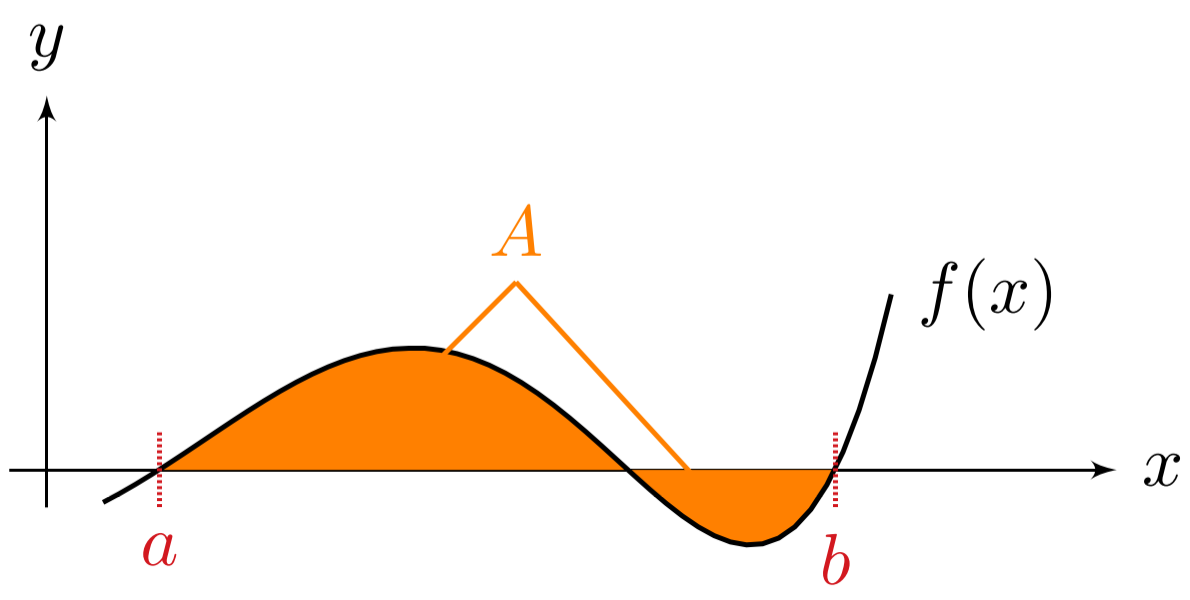
\includegraphics[height=2.5cm]{bilder/integral_flaeche1.png}
		\end{minipage}
		\begin{minipage}{.5\textwidth}
			$A=\int\limits_{a}^{b}\left[f_{1}(x)-f_{2}(x)\right] d x \quad$ für $f_{1}(x) \geq f_{2}(x)$\\
			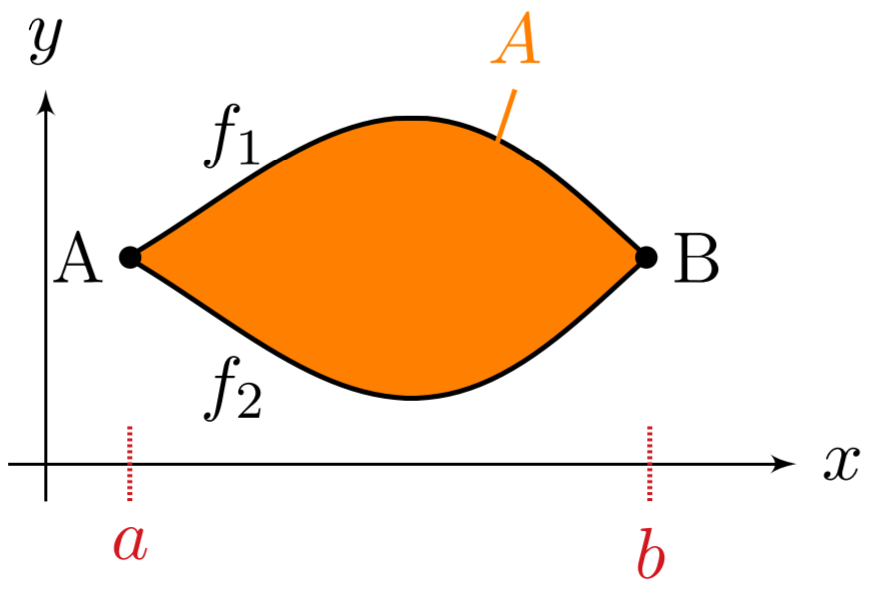
\includegraphics[height=2.5cm]{bilder/integral_flaeche2.png}
		\end{minipage}
